% Chapter Template

\chapter{Results} % Main chapter title
\label{chap:results}


%B-Feld. Von welchem Instrument? auch RTN-System. Genauso Winkel berechnet.
%1-min-Mittel (Gyroradius Zeit zeigen) und entsprechend EpQ-Steps den PHAs zugeordnet.

%
%
%
Todo:\\
Schreiben, dass die velocity Akzeptanzpunkte mit den anteilmäßigen Counts histogrammiert werden? Vielleicht auch ins Data-Kapitel, weil das mit der Normierung gemacht wird...? Sind die Counts überhaupt durch n geteilt?\\ \\
\textbf{Steps vsw, asp...?}
\\ \\ \\
Here we present the results of the procedure described in chapter \ref{chapter:data}. For creating HE+ VDs from He+ SWICS PHA data we synchronize the selected data (s. \ref{chapter:instrumentation} (triple coincidences) with the SC AA, eigen-velocity and solar wind speed.
This gives us directionally resolved counts from the observed phase space volume.
\\
An example for todo days bla is shown in fig. \ref{fig:counts_50}. Here we histogrammed the counts by utilizing cartesian $w_R$, $w_T$ and $w_N$ bins in solar wind frame. Shown are counts in the $w_T - w_N$ plane from a ``slice'' that has been cut out in $w_R$ direction. The orientation of such a cut is sketched in fig. \ref{fig:sketch_slice_R}. In fig. \ref{fig:counts_50} counts within the range $0.3 <= w_R < 0.5$ have been summarized for each $w_T - w_N$ bin.
(D.h. bei vsw ...)
\\
Dividing the counts by the integrated phase space volume for the observed time, which is binned in the same way and shown in fig. \ref{fig:norm_50}, gives the resulting phase space density, s. fig. \ref{fig:psd_50}.\\
When Comparing the three figures one can see a change in shape between phase space volume and phase space density (resp. counts). The phase space density does not cover all of the scanned phase space volume. This means that SWICS did not observe He+ pickup ions over all of the observed phase space volume but only in a distinct partial volume.\\ 
The non-zero parts of phase space density show as a roundish shape in the 2d projection in fig todo. In fact, it is a spherical shape in 3D. As a visualization a stepwise sequence of $w_T - w_N$ ``slices'' is shown in the appendix. Each slice is again a projection of the psd from a width $\Delta w = 0.2$. The sequence starts at about solar wind speed with the slice $-0.1 <= w_R < 0.1 todo$ and steps seamlessly up to $0.9 <= w_R < 1.1$ in todo increments. The radius of the projection decreases towards larger $w_R$ which suggests the 3d shape of a sphere centered around $w_R = 0$.
For $w_R < 0$ and towards smaller values of $w_R$ an increasing ``hole'' in the phase space density emerges from the center. This is due to the fact of a limited instrumental coverage for He at higher ESA steps, which is described in more detail in todo.\\ The same shape shows up when taking slices in the other two dimensions. Verweis auf beide Spektren und die Skizzen.\\

Looking again at the $0.9 <= w_R < 1.1$ slice in fig todo one observes.
Also, the psv shosw a deutlich, schmalen peak in the bins around wT = todo and wN = todo. This means that this part of ps has been observed more often than surrounding parts. This is due to the fact that the spacecraft had a substantial (?) aspect angle (vgl bild bla) in this period of time. Which means that the sc's spin axis for most of the time was tilted away from the radial direction which is reflected by the fact that the peak is shifted a little bit away form the center.The fact that this distinct psv has been observed especially often is followed by a qualitatively similar peak in counts (s. fig todo). 
This is a result of the measurement and not a feature in the velocity distribution of he+. In PSD that feature has vanished, which shows the importance of normalization process. The PSD shows an increased density over a wider range around the radial direction, majority streams central in this example. \\ \\
In fig todo we show the psd for another longer time period todo for slice todo at vsw todo. Here, the counts show a ring structure which vanishes by normalization. 
The PSD in fig todo shows a similar distribution like the psd from the other time period, concentrated and symmetrical around central direction.
\\ \\
We can also choose another (polar) projection. For this we consider spherical shells of constant $w$ in sw frame. Visualization: fig todo: 2d projection of such a concentric shell around w = 0 is shown. Irgendwo Winkel einzeichnen oder erklären.
Zeige beispielhaft Counts und PSV für Zeitraum todo... Auch hier zeigt sich (noch deutlicher) ein helles Feature, was der gebiasten Guckrichtung geschuldet ist. Wenn wir das mithilfe der Normalizierung wegmachen, sehen wir eine andere Verteilung. Für ISotropie müsste alles gleich gefüllt sein, ist es aber nicht.
This projection is capable to visualize features like an anisotropic distribution like the rings, s. theorie
\\ \\
In fig todo haben wir die 3d Verteilung noch mehr runter projiziert: Auf 1D-Spektren. Das entsteht durch integration over spherical shells der Breite todo (für counts und psv). The histogram shows the average psd for shells of different radii.
Wir haben zwei Zeiträume ausgewählt: bla und bla.
Qualitativ ähnlich: CutOff, einigermaßen konstant bis etwa 0.5. Weiter können wir nicht gucken wegen Einschränkung der Coverage (?? vsw gleich? checken...)
\\
Qualitativ ist das auch mit Glöckler vergleichbar, allerdings auf einem ganz anderen Weg entstanden.






\clearpage
\subsection{Slices}


%%% R %%%

\begin{figure}[h]
	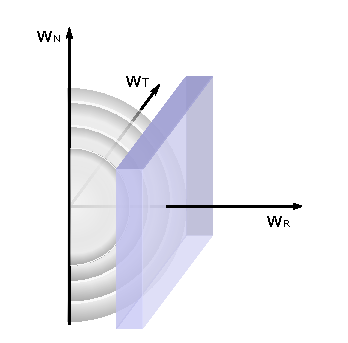
\includegraphics[width=.4\textwidth]{Figures/sketch_slice_R2.pdf}
	\centering
	\caption{todo}
	\label{fig:sketch_slice_R}
\end{figure}


\begin{figure}
	\centering
	\begin{subfigure}{.5\textwidth}
		\centering
		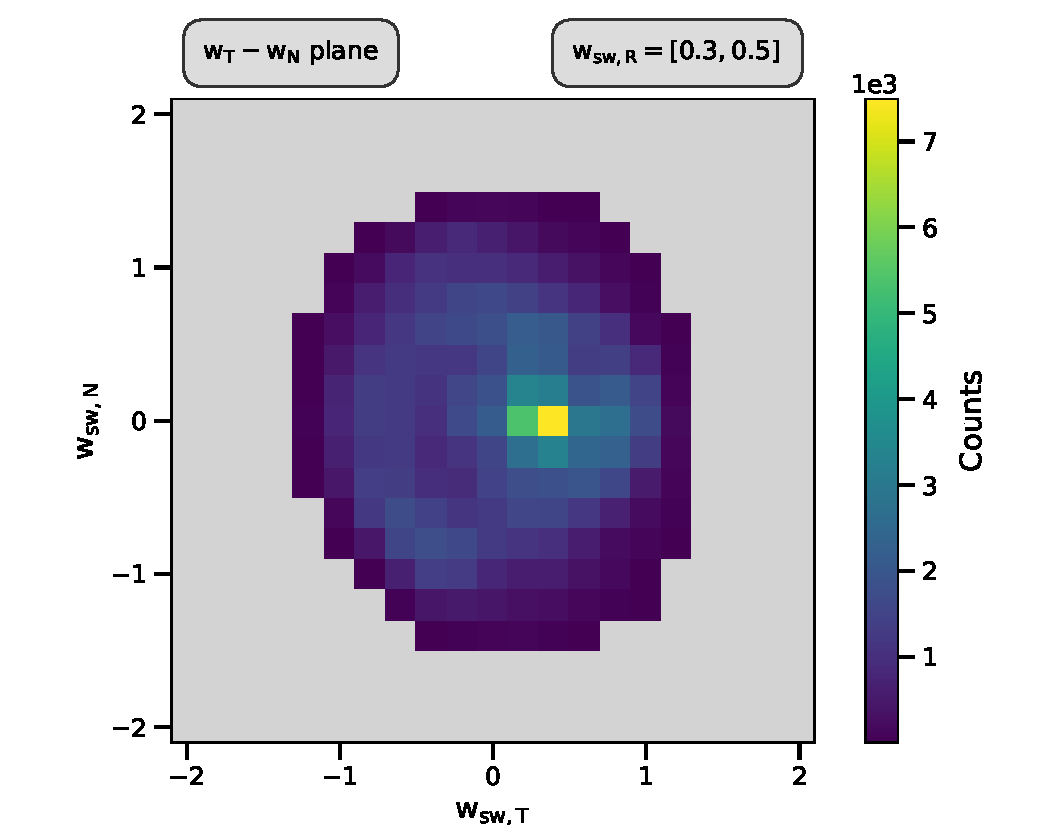
\includegraphics[width=1\textwidth]{Figures/slice_50_counts.pdf}
	\end{subfigure}%
	\begin{subfigure}{.5\textwidth}
		\centering
		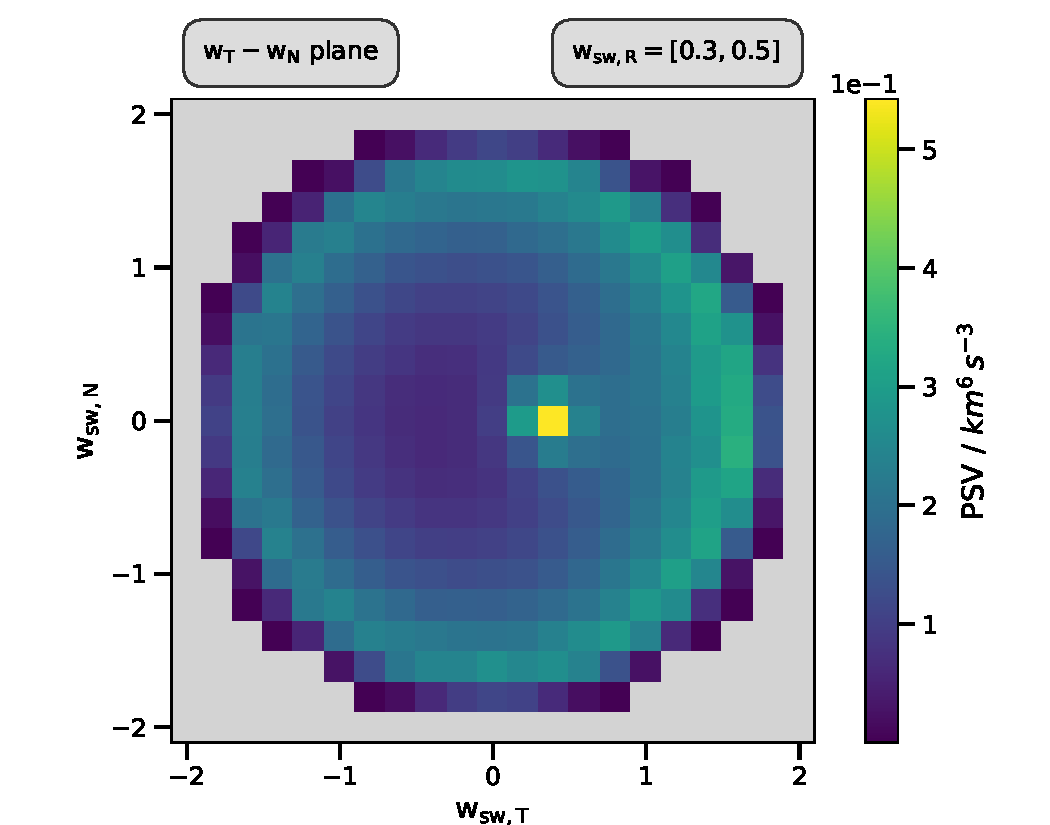
\includegraphics[width=1\textwidth]{Figures/slice_50_norm.pdf}
	\end{subfigure}
	\caption{ring in norm due to psv auf anderen Schalen; da größere Volumina wegen v}
	\label{fig:counts_norm_50}
\end{figure}



\begin{figure}[h]
	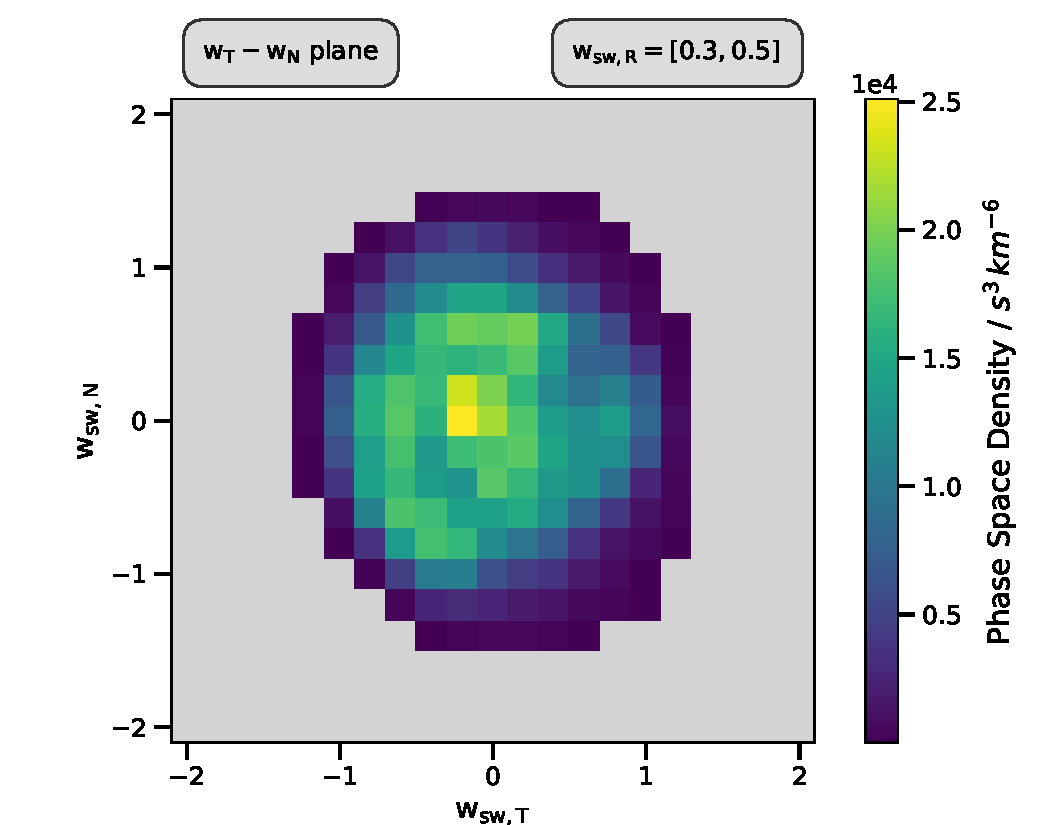
\includegraphics[width=.8\textwidth]{Figures/slices_50_3.pdf}
	\centering
	\caption{todo}
	\label{fig:psd_50}
\end{figure}


\begin{figure}
	\centering
	\begin{subfigure}{.5\textwidth}
		\centering
		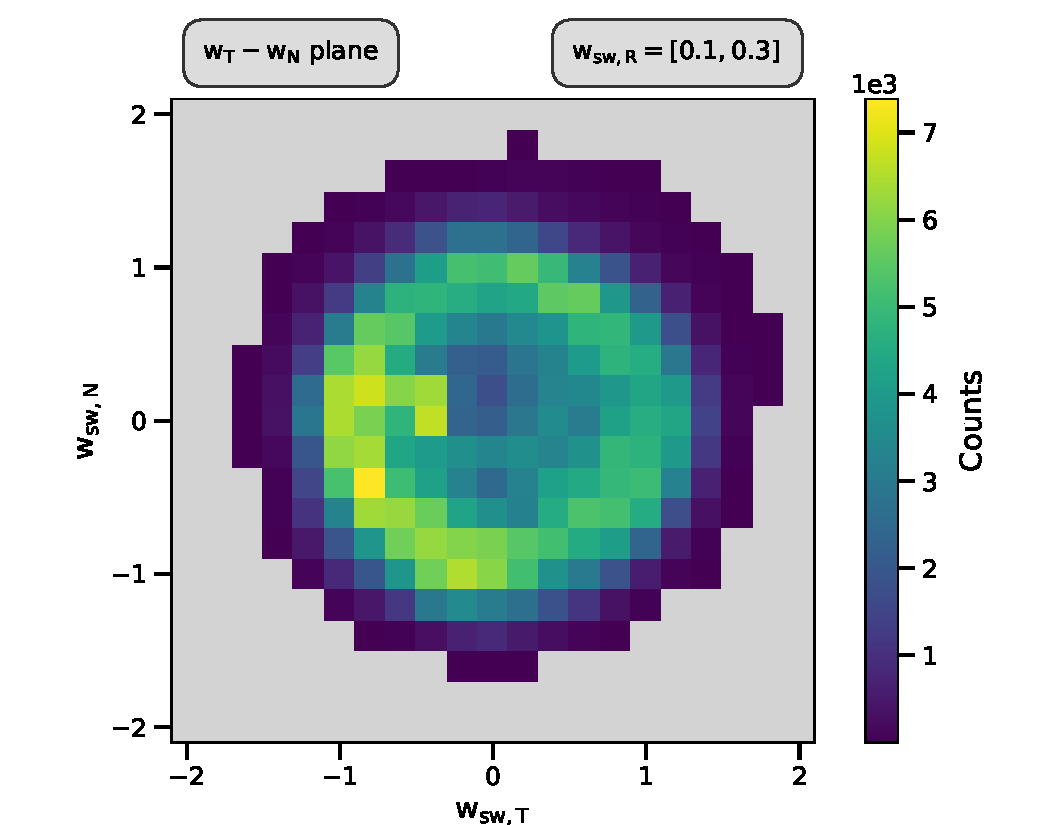
\includegraphics[width=1\textwidth]{Figures/cart_long_counts.pdf}
	\end{subfigure}%
	\begin{subfigure}{.5\textwidth}
		\centering
		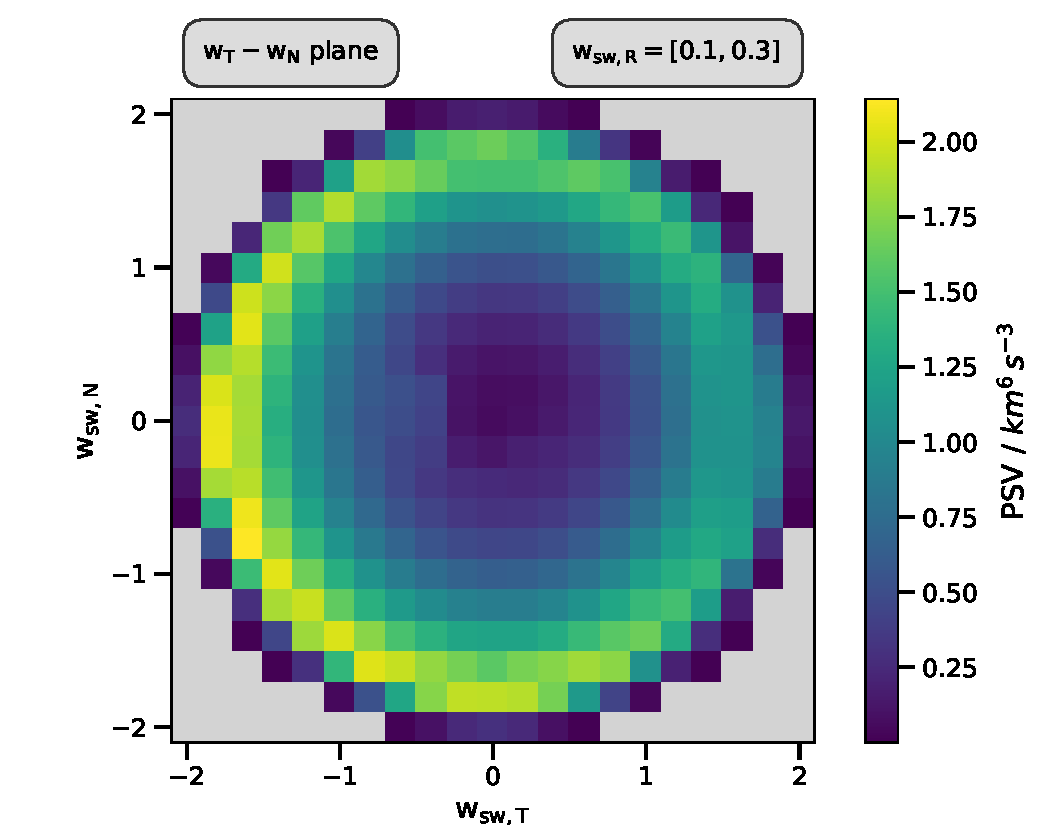
\includegraphics[width=1\textwidth]{Figures/cart_long_norm.pdf}
	\end{subfigure}
	\caption{todo}
	\label{fig:counts_norm_lang}
\end{figure}


\begin{figure}[h]
	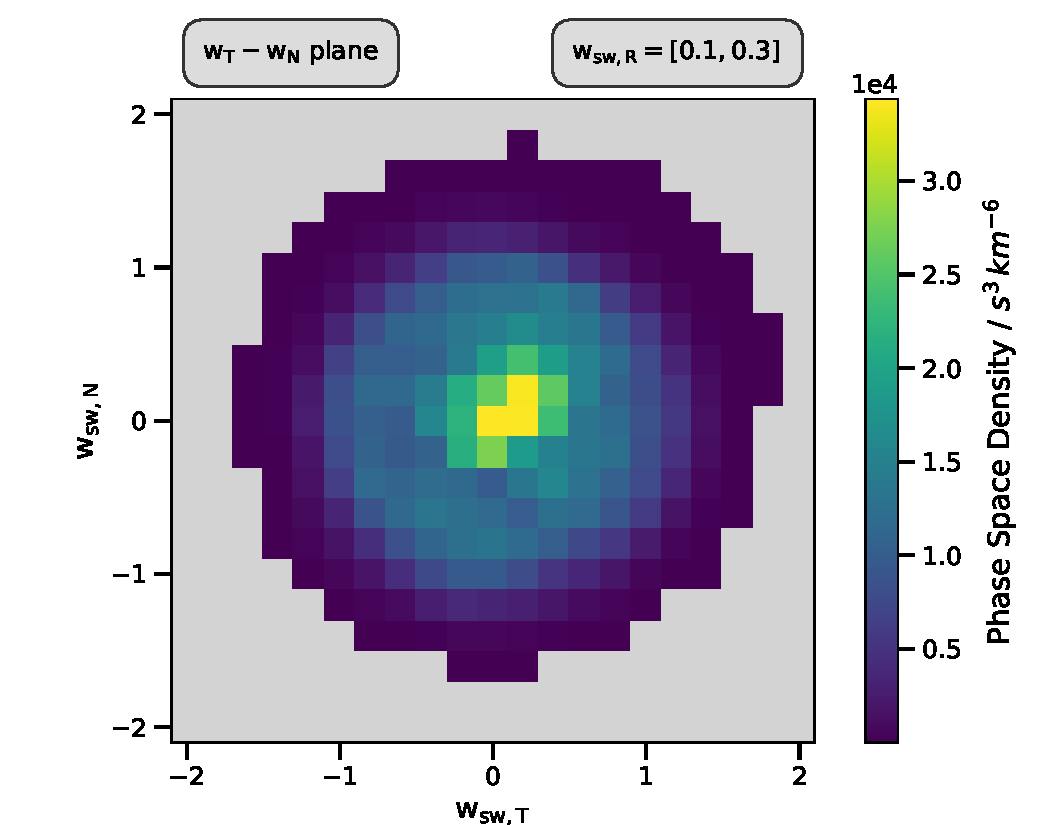
\includegraphics[width=.8\textwidth]{Figures/cart_long_ps.pdf}
	\centering
	\caption{todo}
	\label{fig:psd_lang}
\end{figure}






%%% T %%%
\begin{figure}[h]
	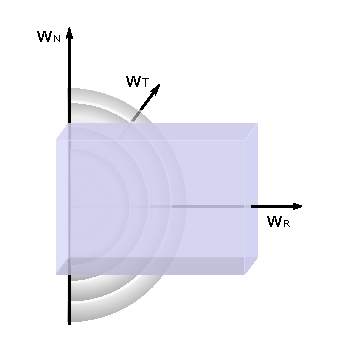
\includegraphics[width=.4\textwidth]{Figures/sketch_slice_T2.pdf}
	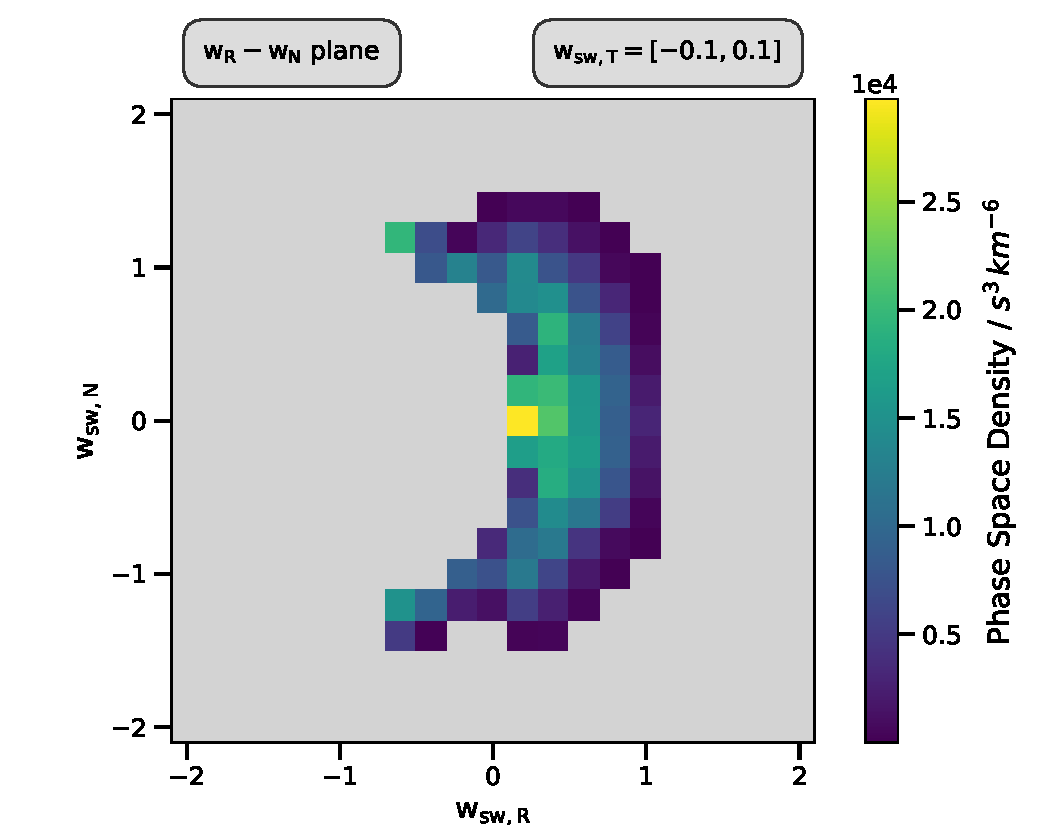
\includegraphics[scale=.45]{Figures/slice_50_T.pdf}
	\centering
	\caption{todo}
	\label{fig:sketch_slice_T}
\end{figure}

%%% N %%%

\begin{figure}[h]
	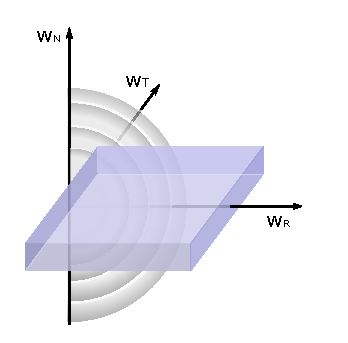
\includegraphics[width=.4\textwidth]{Figures/sketch_slice_N2.pdf}
	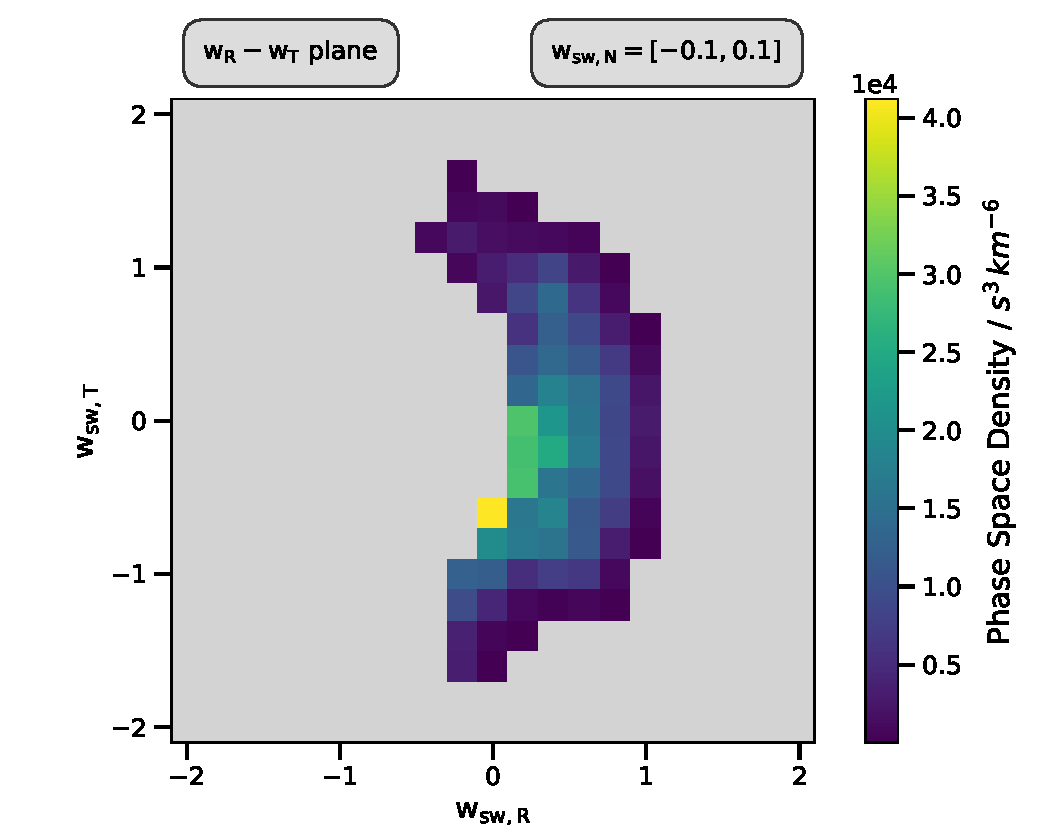
\includegraphics[scale=.45]{Figures/slice_50_N.pdf}
	\centering
	\caption{todo}
	\label{fig:sketch_slice_N}
\end{figure}


%
%
%
\clearpage
\subsection{Skymaps}
\begin{figure}[h]
	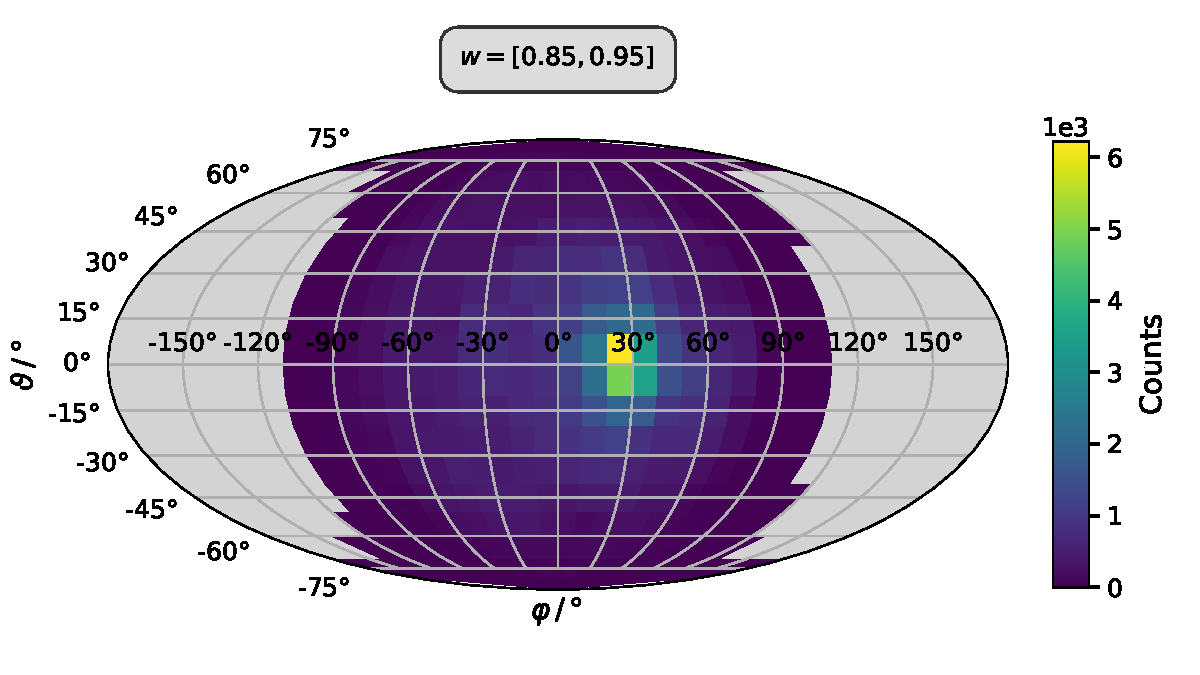
\includegraphics[width=1\textwidth]{Figures/sky_counts.pdf}
	\centering
	\caption{todo}
	\label{fig:todo}
\end{figure}
\begin{figure}[h]
	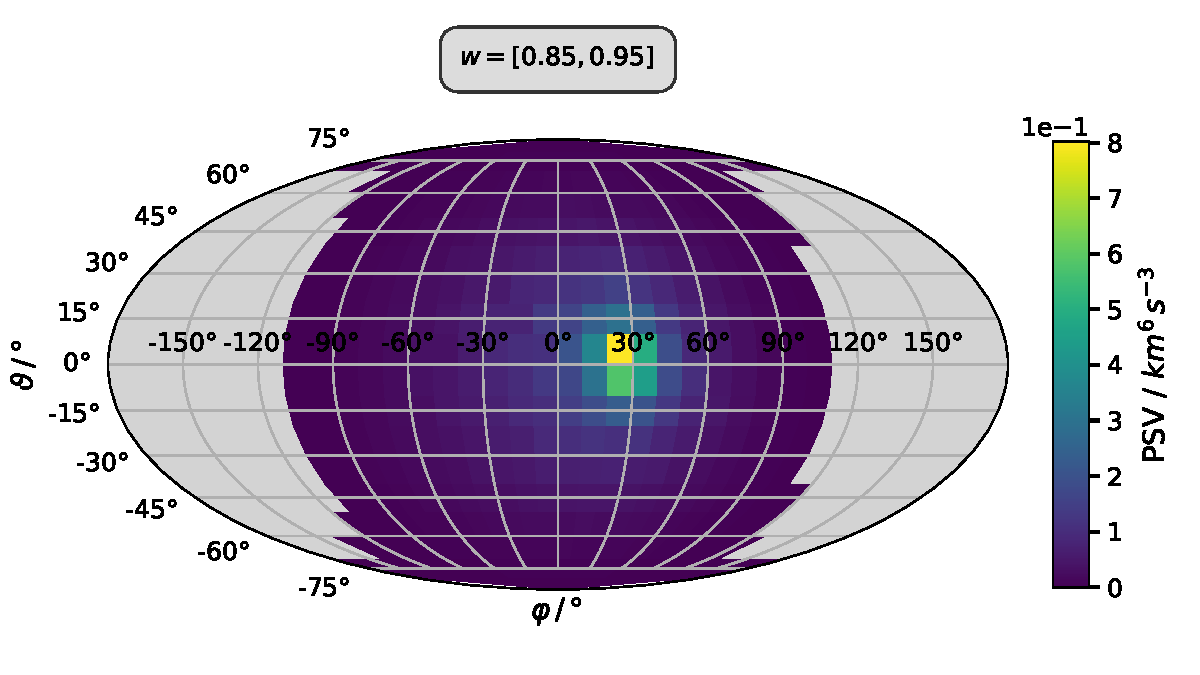
\includegraphics[width=1\textwidth]{Figures/sky_norm.pdf}
	\centering
	\caption{todo}
	\label{fig:todo}
\end{figure}
\begin{figure}[h]
	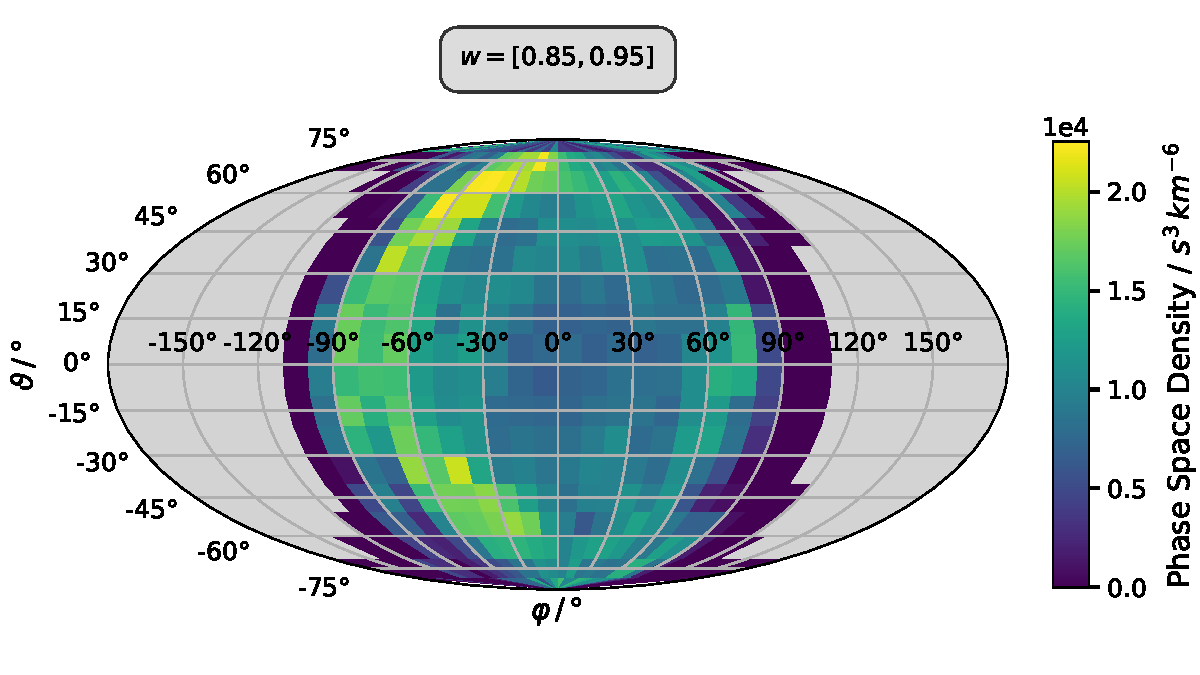
\includegraphics[width=1\textwidth]{Figures/sky_ps.pdf}
	\centering
	\caption{todo}
	\label{fig:todo}
\end{figure}
%
%
%
\clearpage
\subsection{1D}

\begin{figure}[h]
	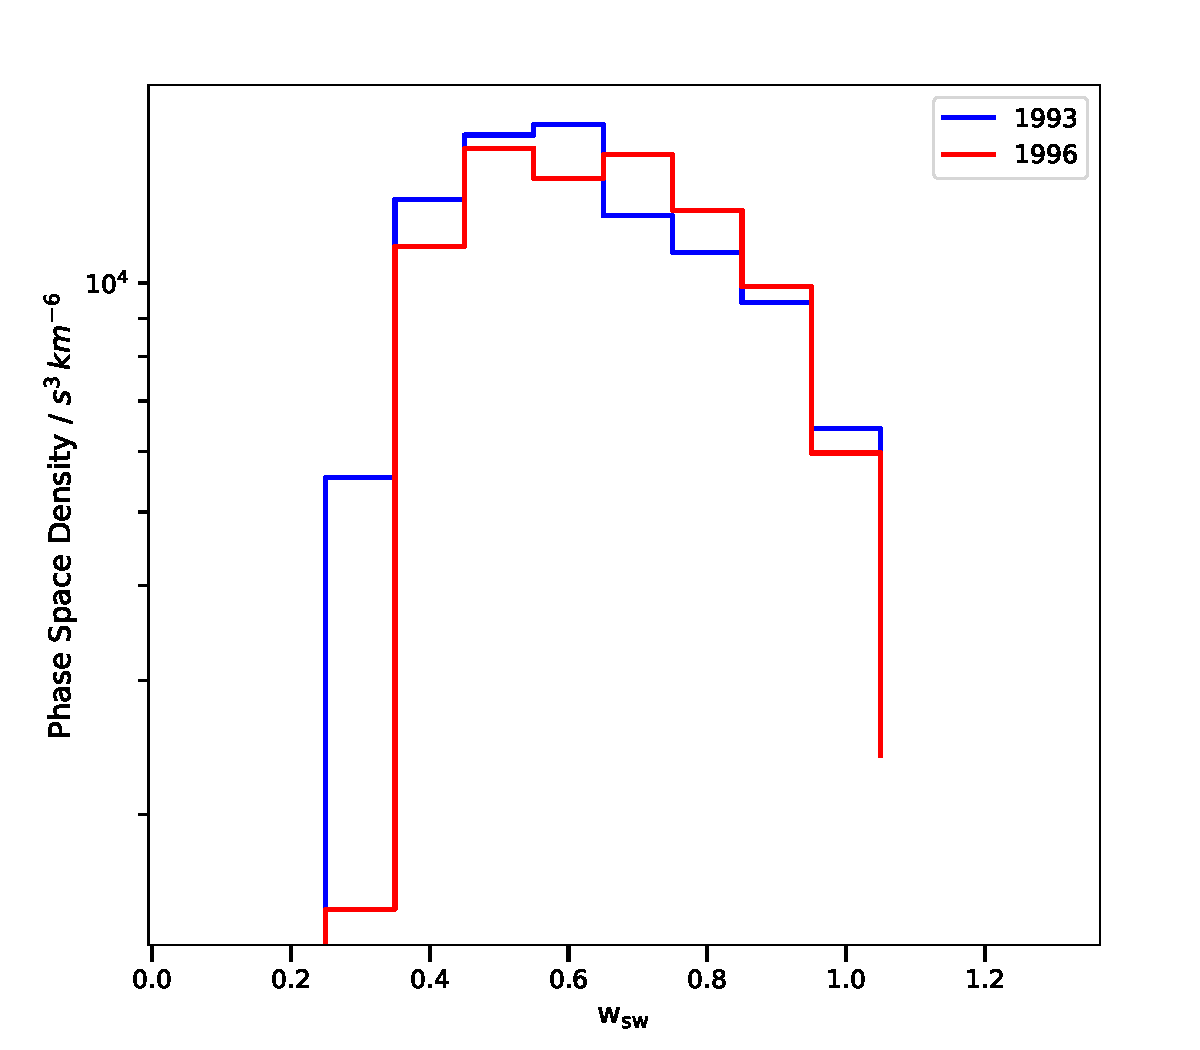
\includegraphics[width=.8\textwidth]{Figures/1D.pdf}
	\centering
	\caption{todo}
	\label{fig:todo}
\end{figure}
%
%
%
\clearpage
\section{Loose Ends}
\begin{itemize}
	\item andere Daten: B, vsw (Swoops: als vsw wird Protonengeschw. genommen. Ist das überhaupt richtig, ist das der Referenzframe? Und Annahme, dass vsw rein radial ist)
	\item Die Sache mit dem BRW ab 2003
	\item Englisch: Relativpronomen, Kommasetzung, British/American
	\item $\mathrm{He^{+}}$ einheitlich, mathrm
	\item Tempus?
	\item kursiv / nicht kursiv wie war das nochmal
	\item spinrate drin?
\end{itemize}
